\chapter{Conculusion and Future Prospects} \label{chap6}
In this chapter, we conclude the thesis and describe future prospects.

\section{Conclusion}
In this study, we developed the baseline compensation system for reducing the influence of the low-frequency seismic noise. The baseline compensation system is the active baseline seismic isolation system for the optical arm cavities. This system only uses the GIF which can measure the baseline length changes directly. The conventional system uses a seismometer to measure the length change, which means that the insufficient isolation performance below 0.1 Hz due to the sensitivity of the seismometer.

We evaluated the performance of the new system by using the X-arm cavity. As a result, we have shown the reduction of the length at least by -6 dB below 1 Hz. The reduction was also in the earth tides band at least by -40 dB. This reduction is the first result of the kilo-meter scale active baseline seismic isolation in the world.

\section{Future Prospects}
In order to obtain higher seismic isolation performance, a seismic isolation system that combines the conventional seismic isolation system and the baseline length compensation system developed in this study is useful.

In this section, we describe the improvement of the baseline compensation system in the future and the prospection of improvement of the duty cycle.

\subsection{Control Design} \label{sec:444}
The demonstration in this study was for 30 minutes, during which the microseismic noise was quiet. In order to improve the duty cycle, it is necessary to isolate the seismic noises even in bad weather. Although we did not implement in this study, it is useful to incorporate a conventional active inertial seismic isolation system so that seismic isolation can isolate the microseismic. In other words, passive seismic isolation using a pendulum is used for frequencies above approximately 1 Hz, a baseline length compensation system is used for frequencies below 1 Hz, and an active inertial vibration isolation system is used for frequencies between 0.1 Hz and 10 Hz. Inertial sensors have higher noise levels than GIFs below 0.1 Hz, but lower levels above that. Therefore, in the microseismic band (0.1 Hz to 1 Hz), the vibration isolation performance of the conventional active inertial vibration isolation system is higher. This conventional system has a narrow frequency band for vibration isolation, but unlike the baseline length compensation system, the common component of the mirrors of the arm cavity can also be isolated. Moreover,  in the microseismic band, the resonance frequency of inverted pendulum exists in the case of KAGRA. Thus the active inertial vibration isolation system using the feedback control is also useful in the point of appropriate damping control of these.

In order to improve the performance of the baseline compensation system, especially the microseismic noise band, we should use the active inertial seismic isolation system to enhance the performance in this band. 

%% \begin{table}[h] 
%%   \begin{center}
%%     \caption{hoge}\label{tb:71}
%%     \begin{tabular}{llllll} 
%%       \hline      
%%       Band [Hz]& $<0.01$ & 0.01 to 0.1 & 0.1 to 1& 1 to 10 & $>10$ \\ \hline \hline
%%       Passive pendulum                         & a & b & c & d & e \\
%%       Active Inertial Seismic Isolation System & a & b & c & d & e \\
%%       Baseline Compensation System             & a & b & c & d & e 
%%     \end{tabular}
%%   \end{center}
%% \end{table}


\begin{figure}[h]
  \begin{center}   
    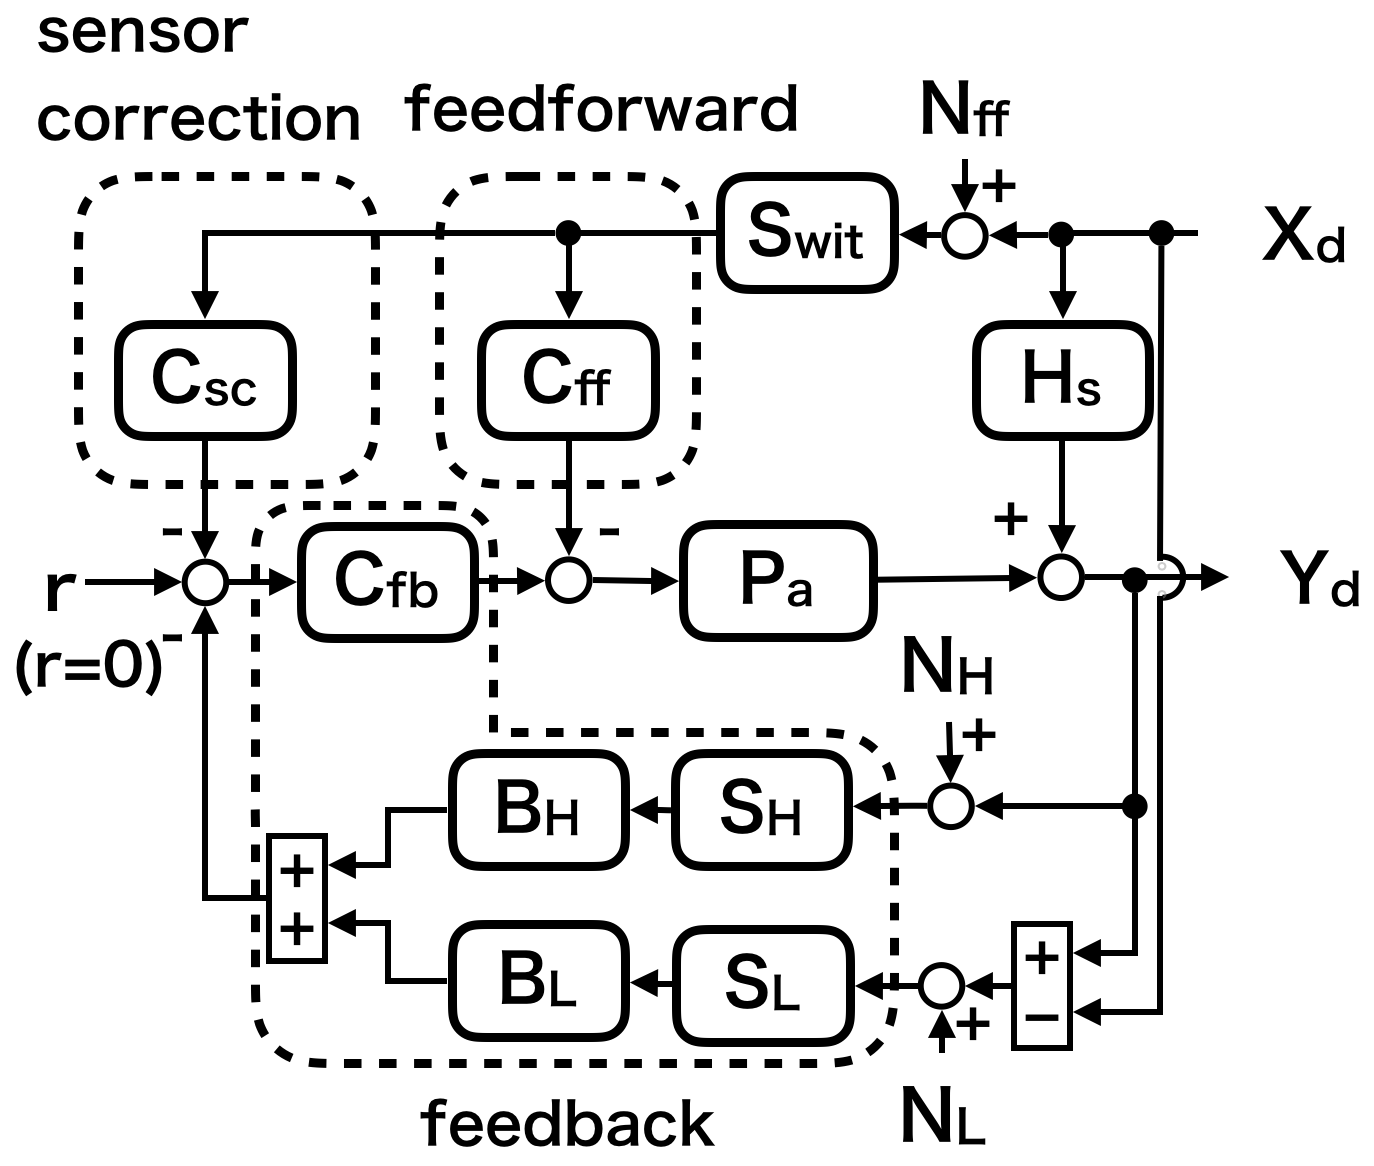
\includegraphics[width=10cm]{./img_chap5/img511.png}
    \caption{The block diagram of the future baseline compensation system.} \label{img:img511}
  \end{center}
\end{figure}

To simplify the discussion, we supposed the CMRR is large enough to ignore the common motion coupling. Thus, we can just consider the only differential component of the motion in this system.

The control diagram of the future baseline compensation system can be represented as shown in Figure \ref{img:img511}. Essentially, all the terms in this figure are the same as the active inertial isolation system shown in Figure \ref{img:img503} except the input and output signals. These signals are replaced as $X_{\mathrm{d}}$ and $Y_{\mathrm{d}}$, which are the differential displacement of the ground and platform stage motions, respectively. In this figure,  $S_{\mathrm{wit}}$ and $N_{\mathrm{ff}}$ are the frequency response and the self-noise of the GIF, respectively. Furthermore, the noises $N_{\mathrm{H}}$ and $N_{\mathrm{L}}$ are multiplied by $\sqrt{2}$ in the case of the amplitude unit.

The displacement of the differential motion of the stages is given by
\begin{eqnarray}\nonumber
  Y_{\mathrm{d}} &=&\frac{G}{1+G}L\Delta_{\mathrm{sc}} X_{\mathrm{d}} + \frac{1}{1+G} \Delta_{\mathrm{ff}} X_{\mathrm{d}}\\ \nonumber
  &+& \frac{G}{1+G}\left(HN_{H}+LN_{L}\right) + \frac{G}{1+G}C_{\mathrm{sc}}S_{\mathrm{wit}}N_{\mathrm{ff}} \\ 
  &+& \frac{1}{1+G}P_{\mathrm{a}} C_{\mathrm{ff}}S_{\mathrm{wit}}N_{\mathrm{ff}} \label{eq:eq520}.
\end{eqnarray}
According to the first and second terms in the equation, the contribution of the ground motion $X_{\mathrm{d}}$ can be independently isolated by three factors: $\Delta_{\mathrm{sc}}$, $\Delta_{\mathrm{ff}}$, and $L$. While the current design needed high loop gain $G$ to reduce the second term, this design does not need due to the $\Delta_{\mathrm{ff}}$. Thus, the feedforward path can make flexible design. Furthermore, the low-pass filter $L$ can isolate the lower frequency motions if the inertial sensor on the stage has enough sensitivity to measure the microseismic noise band.

\subsection{Improvement of Duty Cycle}
If the baseline length compensation system developed in this study is applied to the currently operating gravitational wave detector, it will be possible to improve the lock loss caused by low-frequency ground vibration.

As shown in Figure \ref{img:img190} in chapter \cref{sec:duty}, the low-frequency ground vibration caused by environmental changes causes an average of 10\% lock loss. This method can improve this. Furthermore, because we also reduce the amount of lock loss, we would reduce the number of lock acquisitions. Thus,  locking time, which takes up 20\% of the unobserved state, can also be reduced. Therefore, our compensation system will improve the lock loss except the maintenance or commissioning. The gravitational-wave detectors whose duty cycle is improved will enhance the gravitational-wave astronomy.
